\subsection{Ensayos no destructivos}

\subsubsection{Inspección por líquidos penetrantes (PT)}
\label{sec:pt}

\paragraph{Fundamentos}

El ensayo por líquidos penetrantes es una técnica de ensayos no destructivos de
naturaleza fisicoquímica que permite detectar discontinuidades abiertas a la
superficie en materiales sólidos no porosos \parencite{astm_e165, hull1988}. El
penetrante moja la superficie y entra en la fisura por presión capilar
\parencite{kalinichenko2013}.

Para describir ese ingreso, tómese una fisura idealizada de ancho equivalente $R$ y
profundidad $h$. La ecuación de Rideal--Washburn \parencite{pmc_fluid_mech}
relaciona la profundidad alcanzada con el tiempo de permanencia:

\begin{equation}
  h^2(t) = \frac{\gamma \, R \, \cos\theta}{2\mu}\, t,
  \label{eq:rideal-washburn}
\end{equation}

donde $\gamma$ es la tensión superficial del líquido penetrante ($\text{N/m}$),
$\theta$ el ángulo de contacto dinámico entre el líquido y la pared de la fisura
($\cos\theta > 0$ para que haya mojabilidad), $\mu$ la viscosidad dinámica
($\text{Pa}\cdot\text{s}$) y $t$ el tiempo de permanencia o \textit{dwell time}.
De~\eqref{eq:rideal-washburn} se ve que $h$ crece con la raíz del tiempo: para
duplicar la profundidad hace falta cuadruplicar el tiempo de contacto, y un aumento
de $\mu$ o de $\theta$ frena la penetración. La
Figura~\ref{fig:pt-flujo-capilar} muestra el esquema de la fisura idealizada.

\begin{figure}[H]
  \centering
  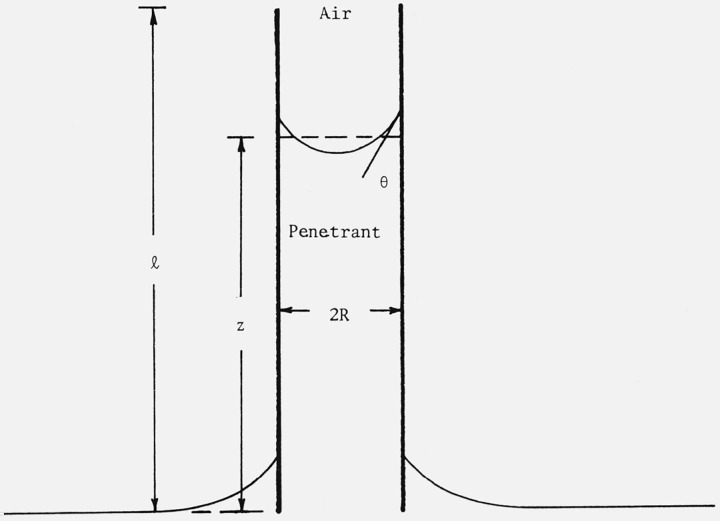
\includegraphics[width=0.55\textwidth]{figuras/deutsch-1979-flujo-capilar.jpg}
  \caption{Flujo capilar del penetrante en un tubo pequeño. Tomado de Deutsch
  (1979).}
  \label{fig:pt-flujo-capilar}
\end{figure}

Retirado el exceso de penetrante de la superficie, se aplica un medio poroso fino
llamado revelador. Éste se comporta como una esponja capilar inversa: absorbe el
líquido que quedó atrapado dentro de la fisura y forma una indicación visible cuyo
tamaño supera con creces el ancho real de la discontinuidad \parencite{almaguer2014}.
Por eso el método alcanza defectos muy por debajo de lo que distingue el ojo. La
Figura~\ref{fig:pt-falla} recoge una falla detectada de este modo en el espécimen 20
ensayado por Almaguer et al. (2014).

\begin{figure}[ht]
  \centering
  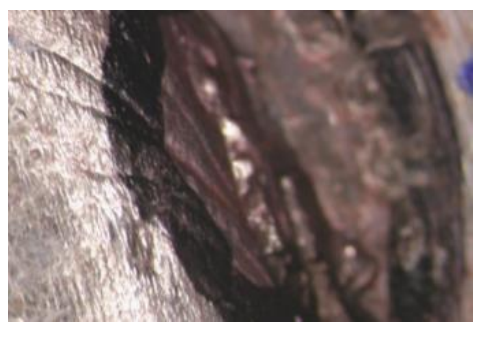
\includegraphics[width=0.42\textwidth]{figuras/almaguer-2014-falla-pt.png}
  \caption{Falla identificada por líquidos penetrantes en el espécimen 20. Adaptado
  de Almaguer et al. (2014).}
  \label{fig:pt-falla}
\end{figure}

\paragraph{Clasificación estandarizada del ensayo (ASTM E1417 / ISO 3452-1)}

De acuerdo con \parencite{astm_e1417, iso3452_1}, el proceso se clasifica según el
tipo de penetrante, el método de remoción del exceso y la forma del revelador.

\begin{enumerate}
  \item \textbf{Por tipo de penetrante:}
  \begin{itemize}
    \item \textbf{Tipo I (fluorescente):} contiene tintes fotosensibles que emiten
          fluorescencia verde-amarilla al excitarlos con radiación UV-A
          ($\lambda = 365\ \text{nm}$). Es el de mayor sensibilidad (niveles
          $1/2$ a $4$).
    \item \textbf{Tipo II (visible):} emplea colorantes rojos intensos que se
          observan con luz blanca natural o artificial ($\ge 1000\ \text{lux}$).
  \end{itemize}
  \item \textbf{Por método de remoción del exceso:}
  \begin{itemize}
    \item \textbf{lavable con agua}: el penetrante lleva agentes emulsionantes
          solubles en agua.
    \item \textbf{post-emulsionable lipofílico}: requiere aplicar después un
          emulsionante a base de aceite.
    \item \textbf{removible con solvente}: se elimina a mano con un paño impregnado
          en solvente no acuoso.
    \item \textbf{post-emulsionable hidrofílico}: usa un emulsionante diluido en agua
          antes del lavado final.
  \end{itemize}
  \item \textbf{Por forma de revelador:}
  \begin{itemize}
    \item polvo seco, aplicado en cámara de suspensión.
    \item soluble en agua.
    \item suspendible en agua.
    \item no acuoso para penetrante tipo I o II (aerosol con base de solvente).
  \end{itemize}
\end{enumerate}

\paragraph{Secuencia operativa estándar}

La inspección cuantitativa sigue seis etapas en orden \parencite{astm_e165}:

\begin{enumerate}
  \item \textbf{Limpieza previa.} Se quitan aceites, grasas, óxidos y pinturas
        mediante desengrase con solvente o ultrasonido.
  \item \textbf{Aplicación del penetrante y tiempo de morada.} Se aplica por
        inmersión, pulverización o pincel y se deja reposar entre $10$ y
        $30\ \text{min}$, según el material.
  \item \textbf{Remoción del exceso.} Se retira el penetrante de la superficie sin
        sacar el que quedó alojado dentro de los defectos.
  \item \textbf{Revelado.} Se extiende una capa delgada de revelador no acuoso
        (forma d) y se deja desarrollar al menos $10\ \text{min}$.
  \item \textbf{Inspección y evaluación.} Las indicaciones se interpretan en
        condiciones controladas: para el tipo II, con iluminación blanca
        $\ge 1000\ \text{lux}$; para el tipo I, con oscuridad ambiental
        ($\le 20\ \text{lux}$) e irradiancia UV-A
        $\ge 1000\ \mu\text{W/cm}^2$ a $38\ \text{cm}$ de distancia. La lámpara
        utilizada se describe en la Sección~\ref{sec:instr-uv}.
  \item \textbf{Limpieza posterior.} Se lava la pieza para evitar corrosión por
        residuos químicos.
\end{enumerate}

El método no detecta discontinuidades cerradas ni internas.

\subsubsection{Inspección por partículas magnéticas (MT)}
\label{sec:mt}

\paragraph{Fundamentos}

La inspección por partículas magnéticas es un END de tipo magnetoelectrostático que
sirve para localizar discontinuidades superficiales y subsuperficiales en materiales
de alta permeabilidad magnética ($\mu_r \gg 1$): aceros al carbono, aceros de baja
aleación y fundiciones ferromagnéticas \parencite{astm_e1444, lovejoy1993}.

El punto de partida es la segunda ecuación de Maxwell, $\nabla \cdot \vec{B} = 0$,
que descarta la existencia de monopolos magnéticos \parencite{rao2012}. Si se induce
un flujo $\Phi$ en una pieza ferromagnética mediante una fuerza magnetomotriz
$\mathcal{F} = N I$, la reluctancia del circuito sigue la ley de Hopkinson
\parencite{lovejoy1993}:

\begin{equation}
  \mathcal{F} = \Phi\,\mathcal{R},
  \qquad
  \mathcal{R} = \frac{l}{\mu_0\,\mu_r\,A},
  \label{eq:hopkinson-reluctancia}
\end{equation}

donde $l$ es la longitud del trayecto magnético, $A$ el área de la sección
transversal, $\mu_0 = 4\pi\times10^{-7}\ \text{H/m}$ la permeabilidad del vacío y
$\mu_r$ la permeabilidad relativa ($100 \le \mu_r \le 5000$).

Cuando el flujo cruza perpendicularmente una fisura de apertura $w$ llena de aire o
de contaminantes ($\mu_{aire}\approx 1$), la reluctancia local sube de golpe
($\mathcal{R}_{grieta} \gg \mathcal{R}_{mat}$). Ese gradiente obliga a las líneas de
campo a deformarse y a salir por la superficie, lo que produce un campo disperso
conocido como fuga de flujo magnético (\textit{Magnetic Flux Leakage}, MFL)
\parencite{rao2012}. Las partículas ferromagnéticas que se espolvorean encima son
atraídas hacia las zonas de mayor gradiente de $|\vec{B}|^2$ por la fuerza Kelvin:

\begin{equation}
  \vec{F}_m = \frac{V_p\,\chi_m}{\mu_0}\,\nabla |\vec{B}|^2,
  \label{eq:fuerza-kelvin}
\end{equation}

con $V_p$ el volumen de la partícula y $\chi_m$ su susceptibilidad magnética.

\begin{figure}[ht]
\centering
\begin{tikzpicture}[scale=0.9]
  % pieza ferromagnética
  \fill[gray!12] (0,0) rectangle (8,2);
  \draw[thick] (0,0) rectangle (8,2);

  % líneas de campo dentro de la pieza
  \foreach \y in {0.3,0.7,1.1,1.5,1.9} {
    \draw[-{Stealth}] (0.25,\y) -- (7.75,\y);
  }

  % grieta llena de aire
  \fill[white] (3.85,0.8) rectangle (4.15,2);
  \draw[thick] (3.85,2) -- (3.85,0.8) -- (4.15,0.8) -- (4.15,2);

  % fuga de flujo magnético
  \draw[-{Stealth}] (3.85,2) .. controls (3.35,2.9) and (4.65,2.9) .. (4.15,2);
  \draw[-{Stealth}] (3.85,2) .. controls (3.55,3.45) and (4.45,3.45) .. (4.15,2);

  % yugo
  \draw[very thick] (1.5,2) -- (1.5,3.6) -- (6.5,3.6) -- (6.5,2);

  % bobina sobre la barra superior
  \foreach \x in {3.0,3.3,...,5.0} {
    \draw[thick] (\x,3.6) -- (\x,3.95);
  }
  \draw[thick] (2.9,3.95) -- (5.1,3.95);

  % partículas magnéticas
  \foreach \p in {(3.6,2.1),(3.75,2.22),(4.25,2.24),(4.4,2.1),(3.5,2.02),(4.5,2.02)} {
    \fill \p circle (0.05);
  }

  % etiquetas
  \node[left] at (1.35,2.9) {yugo};
  \node at (4,4.15) {bobina};
  \node[right,fill=white,inner sep=1pt] at (4.3,0.95) {grieta};
  \node[right,font=\small] at (4.85,2.55) {partículas};
  \draw[-{Stealth},thin] (4.85,2.5) -- (4.55,2.2);
  \node[below] at (4,-0.1) {pieza ferromagnética};
\end{tikzpicture}
\caption{Esquema del ensayo por partículas magnéticas: el yugo magnetiza la pieza,
la grieta distorsiona el campo y las partículas se acumulan en la fuga de flujo.}
\label{fig:mt-esquema}
\end{figure}

\paragraph{Efecto piel y selección del tipo de corriente}

La profundidad con que el campo entra en el material depende de la frecuencia $f$ de
la corriente de magnetización, por el efecto piel. Esa profundidad se estima como
\parencite{rao2012}

\begin{equation}
  \delta = \sqrt{\frac{\rho}{\pi f \mu_0 \mu_r}},
  \label{eq:efecto-piel}
\end{equation}

donde $\rho$ es la resistividad del material ($\Omega\cdot\text{m}$).

\begin{itemize}
  \item \textbf{Corriente alterna (AC, $50/60\ \text{Hz}$).} Como $\delta \approx
        1\ \text{mm}$ en aceros, el campo se queda en la capa superficial y da la
        mayor sensibilidad para fisuras por fatiga abiertas a la superficie.
  \item \textbf{Corriente continua (DC) o rectificada de media onda (HWDC).} Al
        anular la frecuencia ($f\to 0$), el campo penetra en toda la sección y
        permite detectar fisuras subsuperficiales de hasta $3$ a $6\ \text{mm}$.
\end{itemize}

\paragraph{Clasificación estandarizada y métodos (ASTM E1444 / ISO 9934-1)}

Según \parencite{astm_e1444, iso9934_1, asme_bpvc_v}, las técnicas de magnetización
y los medios de detección se ordenan así:

\begin{enumerate}
  \item \textbf{Técnicas de inducción del campo:}
  \begin{itemize}
    \item \textbf{Magnetización longitudinal (yugo o bobina):} el campo va paralelo
          al eje del yugo o del solenoide y detecta grietas transversales a ese eje.
    \item \textbf{Magnetización circular (paso de corriente o conductor central):}
          la corriente circula por la pieza o por un conductor central y genera un
          campo anular, apto para fisuras longitudinales.
    \item \textbf{Magnetización multidireccional:} aplica campos cruzados en
          secuencias rápidas y cubre cualquier orientación en una sola operación.
  \end{itemize}
  \item \textbf{Medios de detección:}
  \begin{itemize}
    \item \textbf{Método seco:} partículas finas de hierro u óxidos coloreados
          (negro, rojo, amarillo) sopladas con aire; sirve para campo y piezas
          rugosas o soldaduras.
    \item \textbf{Método húmedo:} partículas en suspensión en aceite ligero o en
          agua con inhibidor de corrosión.
  \end{itemize}
  \item \textbf{Contraste y visualización:}
  \begin{itemize}
    \item \textbf{Visibles:} se inspeccionan con luz blanca intensa
          ($\ge 1000\ \text{lux}$).
    \item \textbf{Fluorescentes:} llevan pigmentos que emiten verde-amarillo bajo
          UV-A ($\lambda = 365\ \text{nm}$).
  \end{itemize}
\end{enumerate}

\paragraph{Verificación del yugo y secuencia operativa}

El yugo empleado se describe en la Sección~\ref{sec:instr-yugo}. La validez del
ensayo exige comprobar periódicamente su fuerza (\textit{Yoke Lift Test})
conforme a ASTM E1444 \parencite{astm_e1444}:

\begin{itemize}
  \item \textbf{Yugo de AC:} debe levantar una placa patrón de acero de al menos
        $4.5\ \text{kg}$ ($10\ \text{lb}$) con la separación de polos de trabajo.
  \item \textbf{Yugo de DC:} debe levantar al menos $18.1\ \text{kg}$
        ($40\ \text{lb}$).
\end{itemize}

La secuencia estándar tiene estas fases \parencite{iso9934_1}:

\begin{enumerate}
  \item \textbf{Preparación de la superficie.} Se limpian grasa, escamas de
        laminación, pintura suelta y residuos magnéticos.
  \item \textbf{Posicionamiento del yugo y magnetización.} Los polos se apoyan
        perpendiculares a la dirección esperada de la grieta.
  \item \textbf{Aplicación continua de partículas.} El medio húmedo o seco se
        dispersa mientras la corriente sigue activa (\textit{método continuo}).
  \item \textbf{Inspección visual y evaluación.} Con partículas visibles se requiere
        $\ge 1000\ \text{lux}$; con fluorescentes, oscuridad ambiental
        $\le 20\ \text{lux}$ e irradiancia UV-A
        $\ge 1000\ \mu\text{W/cm}^2$ a $38\ \text{cm}$.
  \item \textbf{Desmagnetización residual.} Se aplica un campo alterno decreciente e
        invertido para bajar la inducción remanente de $0.3\ \text{mT}$
        ($3\ \text{Gauss}$) \parencite{astm_e1444}.
\end{enumerate}

El yugo solo es aplicable a materiales ferromagnéticos y exige desmagnetización
posterior \parencite{astm_e1444}.

\subsubsection{Inspección por ultrasonido (UT) y medición de espesores}
\label{sec:ut}

\paragraph{Fundamentos}

La inspección por ultrasonido es un método volumétrico de END que se apoya en la
propagación de ondas elásticas de alta frecuencia ($0.5$ a $25\ \text{MHz}$) por
medios sólidos homogéneos \parencite{krautkramer1990, iso16810}.

En un sólido elástico e isótropo, la velocidad de una onda longitudinal $c_L$ depende
del módulo de Young $E$, del coeficiente de Poisson $\nu$ y de la densidad $\rho$
\parencite{cheeke2017}:

\begin{equation}
  c_L = \sqrt{\frac{E(1-\nu)}{\rho(1+\nu)(1-2\nu)}}.
  \label{eq:velocidad-longitudinal}
\end{equation}

Para el acero al carbono a $20\ ^\circ\text{C}$ se tiene $c_L \approx
5920\ \text{m/s}$.

La medición de espesores por eco de pulso (\textit{pulse-echo}) consiste en medir el
tiempo de vuelo de ida y vuelta, $\Delta t$, que tarda el pulso en ir de la superficie
de entrada a la pared posterior (o a una discontinuidad) y volver al receptor
\parencite{astm_e797}:

\begin{equation}
  e = \frac{c_L\,\Delta t}{2}.
  \label{eq:espesor-tof}
\end{equation}

Al llegar a la interfaz entre el material ($Z_1$) y el medio exterior o la grieta
($Z_2$), la onda se refleja y se refracta según la diferencia de impedancia acústica
$Z = \rho c_L$ ($\text{Pa}\cdot\text{s/m}$). El coeficiente de reflexión en
intensidad, en incidencia normal, es \parencite{krautkramer1990}

\begin{equation}
  R = \left(\frac{Z_2 - Z_1}{Z_2 + Z_1}\right)^2.
  \label{eq:coeficiente-reflexion}
\end{equation}

En la interfaz acero-aire ($Z_{acero}\approx 45\times10^6\ \text{Pa}\cdot\text{s/m}$
frente a $Z_{aire}\approx 400\ \text{Pa}\cdot\text{s/m}$), $R\approx 0.9999$: casi
toda la energía ($99.99\%$) vuelve, lo que permite detectar grietas y medir
espesores con buena resolución.

\paragraph{Acoplamiento acústico y transductores piezoeléctricos}

El pulso se genera y se recibe por efecto piezoeléctrico inverso y directo en
cristales sintéticos de titanato zirconato de plomo (PZT) o niobato de litio
\parencite{cheeke2017}.

\begin{itemize}
  \item \textbf{Transductores de elemento dual.} Llevan dos cristales independientes
        sobre suelas en ángulo, uno emisor y otro receptor, separados por una barrera
        de aislamiento acústico. Así se elimina el ruido de campo cercano y la zona
        muerta, lo que mejora la medición de espesores delgados
        ($0.8$ a $50\ \text{mm}$) y la detección de corrosión interna (picaduras)
        \parencite{astm_e797}.
  \item \textbf{Acoplante acústico.} Como el aire en la interfaz sonda-pieza bloquea
        la onda ($R\to 1$), se aplica un fluido o gel (glicerina, gel acuoso o aceite
        mineral) que elimina la película de aire y deja pasar el pulso.
\end{itemize}

\paragraph{Procedimiento de calibración según INACAL PC-029}

La calibración de un medidor digital de espesores por ultrasonido, descrito en la
Sección~\ref{sec:instr-ut}, sigue el procedimiento INACAL PC-029
\parencite{inacal_pc029, astm_e797}:

\begin{enumerate}
  \item \textbf{Ajuste del cero del palpador.} Se compensa el retardo acústico que
        introduce la suela del transductor.
  \item \textbf{Ajuste de la velocidad del sonido.} El instrumento se calibra con un
        bloque patrón de acero a dos espesores acotados, por ejemplo
        $L_1 = 2.5\ \text{mm}$ y $L_2 = 20.0\ \text{mm}$.
  \item \textbf{Verificación de linealidad.} Se evalúan cinco puntos uniformes de un
        bloque patrón escalonado (\textit{step block}) con trazabilidad nacional o
        internacional.
  \item \textbf{Incertidumbre combinada.} Conforme a la guía GUM
        \parencite{jcgm2008gum}, la incertidumbre del espesor medido se compone de
        \begin{equation}
          u_c^2(d) = u^2(\bar{d}_{rep}) + u^2(d_{res}) + u^2(L_{BP})
                     + u^2(\delta c_L) + u^2(\delta T),
          \label{eq:ut-incertidumbre}
        \end{equation}
        donde $u(\bar{d}_{rep}) = s/\sqrt{n}$ es la repetibilidad (tipo A),
        $u(d_{res}) = d_{res}/(2\sqrt{3})$ la resolución del display y
        $u(\delta c_L)$ recoge la variabilidad del material.
\end{enumerate}

\paragraph{Modos de presentación de datos ultrasónicos}

La Figura~\ref{fig:ut-modos} resume los tres modos con que se presenta la señal.

\begin{figure}[ht]
\centering
\begin{tikzpicture}[scale=0.82]
  % (a) A-Scan
  \begin{scope}
    \draw[-{Stealth}] (0,0) -- (4.2,0) node[right,font=\scriptsize] {$t$};
    \draw[-{Stealth}] (0,0) -- (0,2.2) node[above,font=\scriptsize] {$A$};
    \draw[thick] (0.15,0.1) -- (3.9,0.1);
    \draw[thick] (0.35,0.1) -- (0.45,1.55) -- (0.55,0.1);
    \draw[thick] (0.65,0.1) -- (0.8,0.28) -- (0.95,0.08)
                 -- (1.1,0.24) -- (1.25,0.07) -- (1.4,0.2)
                 -- (1.55,0.06) -- (1.7,0.16) -- (1.85,0.05)
                 -- (2.0,0.13) -- (2.15,0.04) -- (2.3,0.1) -- (2.45,0.05);
    \draw[thick] (2.65,0.05) -- (2.75,1.15) -- (2.85,0.05);
    \node[font=\scriptsize] at (2.1,-0.55) {(a) A-Scan};
  \end{scope}

  % (b) B-Scan
  \begin{scope}[shift={(5.3,0)}]
    \fill[gray!12] (0,0) rectangle (4,2);
    \draw (0,0) rectangle (4,2);
    \fill[gray!55] (0,1.55) rectangle (4,1.75);
    \fill[black!80] (2.1,0.55) rectangle (2.45,0.85);
    \draw[-{Stealth}] (0,-0.15) -- (4.2,-0.15) node[right,font=\scriptsize] {$x$};
    \draw[-{Stealth}] (-0.15,0) -- (-0.15,2.15) node[above,font=\scriptsize] {$t$};
    \node[font=\scriptsize] at (2.1,-0.55) {(b) B-Scan};
  \end{scope}

  % (c) C-Scan
  \begin{scope}[shift={(10.6,0)}]
    \fill[gray!10] (0,0) rectangle (4,2);
    \draw (0,0) rectangle (4,2);
    \fill[red!20] (2.0,0.9) circle (0.55);
    \fill[red!60] (2.0,0.9) circle (0.3);
    \draw[-{Stealth}] (0,-0.15) -- (4.2,-0.15) node[right,font=\scriptsize] {$x$};
    \draw[-{Stealth}] (-0.15,0) -- (-0.15,2.15) node[above,font=\scriptsize] {$y$};
    \node[font=\scriptsize] at (2.1,-0.55) {(c) C-Scan};
  \end{scope}
\end{tikzpicture}
\caption{Modos de presentación de datos ultrasónicos: (a) A-Scan, amplitud frente al
tiempo de vuelo; (b) B-Scan, corte transversal con la indicación del defecto;
(c) C-Scan, vista en planta con la posición del reflector.}
\label{fig:ut-modos}
\end{figure}

\begin{itemize}
  \item \textbf{A-Scan (amplitud).} Gráfica unidimensional de la señal RF o
        rectificada: la amplitud del eco ($y$) frente al tiempo de vuelo o la
        distancia ($x$).
  \item \textbf{B-Scan (corte transversal).} Representación bidimensional del perfil
        de la pieza a lo largo de una línea de escaneo; sirve para ver mapas de
        corrosión y pérdida de pared.
  \item \textbf{C-Scan (vista de planta).} Mapeo en el plano $x$-$y$ que muestra la
        profundidad o la amplitud de los reflectores en toda el área inspeccionada.
\end{itemize}

\subsubsection{Inspección visual (VT)}
\label{sec:vt}

\paragraph{Fundamentos}

La inspección visual es el método primario de los END: se realiza antes que cualquier
otra técnica, superficial o volumétrica, y no necesita equipos especiales
\parencite{asme_bpvc_v_art9, iso17637}. Se apoya en la interacción de la luz visible
($\lambda \in [380,780]\ \text{nm}$) con la superficie de la pieza y en la respuesta
del ojo o de un sensor electroóptico \parencite{moore2012}.

La iluminación que llega al inspector sigue la ley del inverso del cuadrado de la
distancia y el teorema del coseno de Lambert \parencite{cheeke2017}:

\begin{equation}
  E_v = \frac{I_v \cos\theta}{r^2},
  \label{eq:iluminancia-lambert}
\end{equation}

donde $E_v$ es la iluminancia sobre la superficie ($\text{lux} = \text{lm/m}^2$),
$I_v$ la intensidad luminosa de la fuente (candela), $r$ la distancia de la fuente al
punto de inspección (m) y $\theta$ el ángulo entre la luz y la normal a la superficie.

La resolución espacial del ojo, $\Delta x_{min}$, se deduce del umbral de agudeza
visual angular $\theta_{min}\approx 1$ minuto de arco $= 2.91\times10^{-4}\ \text{rad}$
\parencite{moore2012}:

\begin{equation}
  \Delta x_{min} = d_{vis}\tan\theta_{min} \approx d_{vis}\,\theta_{min}.
  \label{eq:agudeza-visual}
\end{equation}

A la distancia de visión cercana, $d_{vis} = 250\ \text{mm}$, queda
$\Delta x_{min}\approx 0.07\ \text{mm}$ ($70\ \mu\text{m}$).

\paragraph{Clasificación estandarizada del ensayo (ISO 17637 / ASME Sec. V Art. 9)}

Conforme a \parencite{asme_bpvc_v_art9, iso17637}, la técnica se divide según la
accesibilidad de la pieza:

\begin{enumerate}
  \item \textbf{Inspección visual directa.} Se usa cuando hay línea de visión directa
        e ininterrumpida. Para asegurar la confiabilidad, las normas fijan la
        geometría de observación \parencite{iso17637}:
  \begin{itemize}
    \item \textbf{Distancia de visión:} el ojo no debe estar a más de
          $600\ \text{mm}$ ($24\ \text{pulg}$) de la superficie.
    \item \textbf{Ángulo de visión:} el ángulo entre la línea de visión y el plano de
          la superficie no debe ser menor de $30^\circ$.
    \item \textbf{Instrumentación auxiliar:} lupas de $2\times$ a $10\times$, espejos
          planos articulados, linternas LED de alta intensidad y galgas de soldadura
          (Cambridge, Hi-Lo, escala de filete y micrómetros de profundidad).
  \end{itemize}
  \item \textbf{Inspección visual remota o indirecta (RVT).} Se emplea en cavidades
        internas, tuberías de diámetro reducido, recipientes a presión o zonas de
        alta radiación donde no se puede acceder \parencite{asme_bpvc_v_art9}.
        Usa sistemas ópticos y optoelectrónicos:
  \begin{itemize}
    \item \textbf{Boroscopios rígidos:} lentes acromáticas en tubo metálico con guía
          de luz de fibra óptica; buena resolución angular, pero ángulo de visión
          fijo.
    \item \textbf{Fibroscopios flexibles:} haz de fibras ópticas coherentes para la
          imagen y fibras desordenadas para la iluminación.
    \item \textbf{Videoendoscopios digitales:} cabezales articulados con sensor
          CCD/CMOS en la punta, iluminación LED y procesamiento digital, con
          medición tridimensional por estereofotogrametría o escaneo láser
          \parencite{moore2012}.
  \end{itemize}
\end{enumerate}

\begin{figure}[ht]
\centering
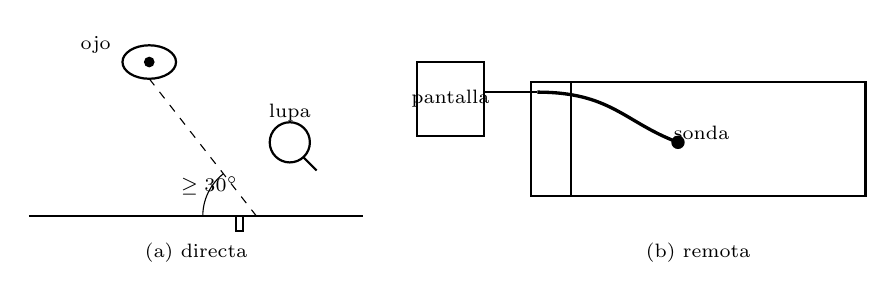
\begin{tikzpicture}[scale=0.85]
  % (a) inspección directa
  \begin{scope}
    \draw[thick] (0,0) -- (5,0);
    \draw[thick] (1.8,2.3) ellipse (0.4 and 0.25);
    \fill (1.8,2.3) circle (0.08);
    \draw[dashed] (1.8,2.05) -- (3.4,0);
    \draw (2.6,0) arc (180:128:0.8);
    \node[font=\scriptsize] at (2.7,0.45) {$\ge 30^\circ$};
    \node[font=\scriptsize] at (1.0,2.55) {ojo};
    % lupa
    \draw[thick] (3.9,1.1) circle (0.3);
    \draw[thick] (4.1,0.88) -- (4.3,0.68);
    \node[font=\scriptsize] at (3.9,1.55) {lupa};
    % defecto superficial
    \draw[thick] (3.1,0) -- (3.1,-0.22) -- (3.2,-0.22) -- (3.2,0);
    \node[font=\scriptsize] at (2.5,-0.55) {(a) directa};
  \end{scope}

  % (b) inspección remota
  \begin{scope}[shift={(7.5,0)}]
    \draw[thick] (0,0.3) -- (5,0.3) -- (5,2) -- (0,2) -- cycle;
    \draw[thick] (0.6,0.3) -- (0.6,2);
    \draw[very thick] (0.1,1.85) .. controls (1.2,1.85) and (1.4,1.4) .. (2.2,1.1);
    \fill (2.2,1.1) circle (0.1);
    \node[font=\scriptsize] at (2.55,1.25) {sonda};
    % cable y pantalla
    \draw[thick] (0.1,1.85) -- (-0.7,1.85);
    \draw[thick] (-1.7,1.2) rectangle (-0.7,2.3);
    \node[font=\scriptsize] at (-1.2,1.75) {pantalla};
    \node[font=\scriptsize] at (2.5,-0.55) {(b) remota};
  \end{scope}
\end{tikzpicture}
\caption{Inspección visual: (a) directa, con la línea de visión y el ángulo mínimo de
observación; (b) remota, con una sonda videoendoscópica en el interior de una
cavidad.}
\label{fig:vt-directa-remota}
\end{figure}

\paragraph{Secuencia operativa en uniones soldadas}

En uniones soldadas de acero estructural o tuberías, la inspección visual se hace en
tres fases \parencite{iso17637}:

\begin{enumerate}
  \item \textbf{Antes del soldeo.} Se verifica el ángulo de bisel, la apertura de
        raíz (\textit{root gap}), la alineación de bordes (\textit{hi-lo}), la
        ausencia de óxido, pintura o humedad y la conformidad de los materiales de
        aporte.
  \item \textbf{Durante el soldeo.} Se revisa la pasada de raíz, la limpieza de
        escoria entre pases y la posible aparición de grietas de solidificación o
        poros.
  \item \textbf{Después del soldeo.} Se evalúan la forma y el sobreespesor del
        refuerzo, las socavaciones (\textit{undercut}), la falta de llenado
        (\textit{underfill}), los traslapes (\textit{overlap}), las porosidades
        abiertas, las salpicaduras (\textit{spatter}) y el socavamiento de raíz.
\end{enumerate}

\paragraph{Requisitos ambientales y calificación del personal}

\begin{itemize}
  \item \textbf{Iluminancia.} ISO 17637 exige al menos $350\ \text{lux}$ sobre la
        superficie para inspección general y recomienda $1000\ \text{lux}$ para
        caracterizar microfisuras \parencite{iso17637}.
  \item \textbf{Calificación del inspector.} Debe acreditar cada año agudeza visual
        cercana con la carta Jaeger N.º 1 (o el equivalente ISO 18490 a
        $30\ \text{cm}$) y distinguir contrastes cromáticos (test de Ishihara),
        conforme a ISO 9712 o ASNT SNT-TC-1A \parencite{iso9712}.
\end{itemize}

